图~\ref{fig:representer-finite-readings-to-solver}串起从有限读取到系数求解的步骤：先删去读数看不见的正交分量，再把读取与范数写成同一个Gram矩阵上的有限表达式。

\begin{figure*}[htbp]
  \centering
  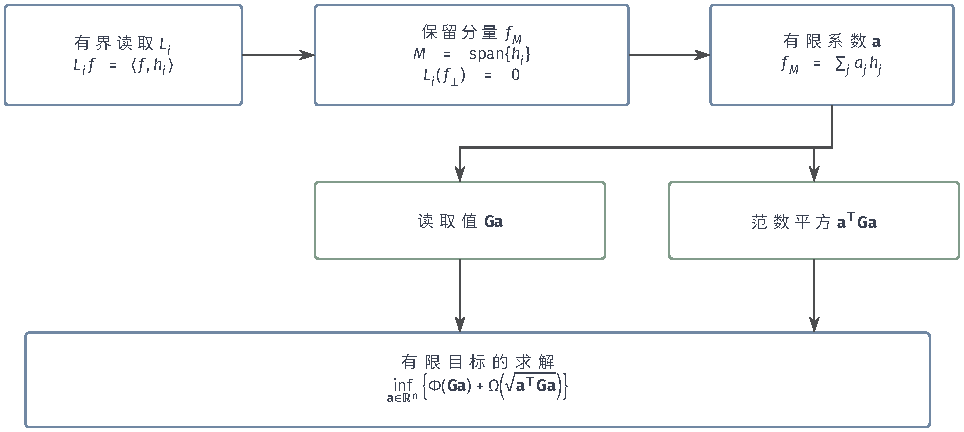
\includegraphics[width=163.258mm]{figures/01-mathematical-preliminaries-upper/00-shared/tikz/representer-finite-readings-to-solver/source.pdf}
  \caption{有限读取下的表示与求解。有界线性泛函$L_i$在Hilbert空间中有Riesz表示元$h_i$。
  所有读取只依赖$M=\operatorname{span}\{h_i\}$中的分量$f_M$，
  单调不减的范数惩罚允许删去$f_\perp$而不增大目标。
  写$f_M=\sum_j a_jh_j$后，读数与范数平方分别为$\bm G\bm a$与$\bm a^\top\bm G\bm a$。
  将这两个有限表达式代入目标后即可求解系数；最优解存在与系数唯一仍需另行判断。}
  \label{fig:representer-finite-readings-to-solver}
\end{figure*}
